\documentclass[10pt,a4paper]{article}

% ─── Packages ─────────────────────────────────────────
\usepackage{fontspec}
\setmainfont{Times New Roman}

\usepackage[top=1.1cm,bottom=1.1cm,left=1.55cm,right=1.55cm]{geometry}
\usepackage{titlesec}
\usepackage{enumitem}
\usepackage{hyperref}
\usepackage{xcolor}
\usepackage{tabularx}
\usepackage{graphicx}
\usepackage{parskip}

% ─── Colors ───────────────────────────────────────────
\definecolor{primary}{RGB}{30,40,90}
\definecolor{namecolor}{RGB}{0,120,180}
\definecolor{accent}{RGB}{50,90,150}
\definecolor{rulecol}{RGB}{200,205,220}
\definecolor{gray}{RGB}{90,90,90}

\hypersetup{
    colorlinks=true,
    urlcolor=accent
}

\pagestyle{empty}
\setlength{\parskip}{0pt}

% ─── Section ──────────────────────────────────────────
\titleformat{\section}
    {\normalsize\bfseries\color{primary}}
    {}
    {0em}
    {}
    [\vspace{1pt}\textcolor{rulecol}{\titlerule[0.6pt]}\vspace{1pt}]

\titlespacing{\section}{0pt}{5pt}{2pt}

% ─── Entry ────────────────────────────────────────────
\newcommand{\entry}[3]{%
    \noindent
    \begin{tabularx}{\linewidth}{X r}
        \textbf{\color{primary}#1} &
        {\scriptsize\color{gray}#2}
    \end{tabularx}\\[-2pt]
    {\scriptsize\textit{\color{gray}#3}}
    \vspace{1pt}
}

% ─── Compact list ─────────────────────────────────────
\newenvironment{cvitems}{
    \begin{itemize}[
        leftmargin=1.15em,
        topsep=0pt,
        itemsep=0.5pt,
        parsep=0pt,
        partopsep=0pt
    ]
}{
    \end{itemize}
}

% ═════════════════════════════════════════════════════
\begin{document}

% ─── HEADER ───────────────────────────────────────────
\noindent
\begin{tabularx}{\linewidth}{@{}X r@{}}

\begin{minipage}[c]{\linewidth}

    {\LARGE\bfseries\color{namecolor} Ho Huynh Nhu}\\[2pt]

    {\large\bfseries\color{primary}
    AI \& Agentic AI}\\[3pt]

    {\scriptsize\color{gray}
    20/10/2003
    \enspace\textcolor{rulecol}{|}
    \enspace (+84) 367 503 477
    \enspace\textcolor{rulecol}{|}
    \enspace
    \href{mailto:hhnhu2003@gmail.com}{hhnhu2003@gmail.com}
    \enspace\textcolor{rulecol}{|}
    \enspace Ho Chi Minh City}\\[2pt]

    {\scriptsize
    \href{https://github.com/hohuynhnhu}
    {github.com/hohuynhnhu}
    \enspace\textcolor{rulecol}{|}
    \enspace
    \href{https://www.facebook.com/huynhnhu.ho.961}
    {facebook.com/huynhnhu.ho.961}
    }

\end{minipage}

&

\begin{minipage}[c]{2.2cm}
    \raggedleft
    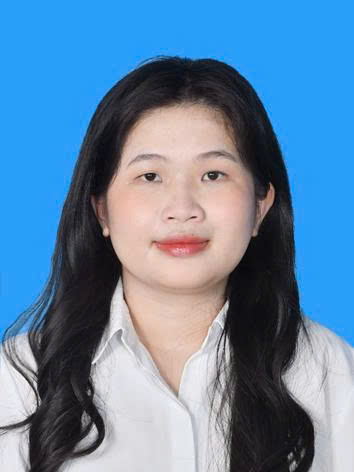
\includegraphics[
        width=2.2cm,
        height=2.7cm,
        keepaspectratio
    ]{assets/avt.jpg}
\end{minipage}

\end{tabularx}

\vspace{3pt}
\textcolor{rulecol}{\rule{\linewidth}{0.6pt}}

% ─── CAREER OBJECTIVE ─────────────────────────────────
\section*{Career Objective}

{\small
Final-year Information Technology student with a strong interest in
Generative AI and Agentic AI, and hands-on experience in LLMs, RAG,
Python, SQL, machine learning, deep learning, APIs, workflow automation,
and BI dashboards. Experienced in building and evaluating AI models and
connecting them with databases and applications. Seeking an AI position
with a ``build and experiment'' mindset to create AI assistants and
automation that save time and support business and sales teams.
}

% ─── EDUCATION ────────────────────────────────────────
\section*{Education}

\entry
{University of Transport Ho Chi Minh City (UTH)}
{10/2022 -- 10/2026}
{Bachelor of Information Technology -- Completed coursework}

{\small
\begin{cvitems}
    \item GPA: 3.4 / 4.0
    \item \textbf{Excellent Scholarship} -- Semester 1, 2025
    \item \textbf{Second Prize -- AI Track},
    UTH Student Scientific Research Conference 2025
\end{cvitems}
}

% ─── TECHNICAL SKILLS ─────────────────────────────────
\section*{Technical Skills}

{\small
\begin{tabularx}{\linewidth}{@{}lX@{}}

\textbf{Generative AI}
&
LLMs, Retrieval-Augmented Generation (RAG)
\\[1pt]

\textbf{AI / Machine Learning}
&
Python, Scikit-learn, EDA, Feature Engineering, Classification,
Regression, Random Forest, Model Evaluation, Cross-Validation
\\[1pt]

\textbf{Deep Learning}
&
PyTorch, CNN, Siamese Network, Transformer,
YOLO, MediaPipe
\\[1pt]

\textbf{APIs \& Automation}
&
FastAPI, RESTful API, Apache Airflow (workflow automation),
RabbitMQ, Power Apps, SharePoint
\\[1pt]

\textbf{Data Engineering}
&
ETL/ELT, Data Pipeline, dbt, Data Lake, Data Warehouse,
Pandas, NumPy
\\[1pt]

\textbf{SQL / Database}
&
SQL, PostgreSQL, SQL Server, MongoDB,
Firebase, Supabase
\\[1pt]

\textbf{Data Visualization}
&
Power BI, Metabase, DAX, Matplotlib, Seaborn
\\[1pt]

\textbf{Programming \& Tools}
&
Python, SQL, TypeScript, JavaScript, Kotlin, Git, Docker, Postman, VS Code

\end{tabularx}
}

% ─── WORK EXPERIENCE ──────────────────────────────────
\section*{Work Experience}

\entry
{Gotik Consulting -- Data Engineer}
{Python \textbar{} dbt \textbar{} PostgreSQL \textbar{} Airflow \textbar{} Power BI}
{03/2026 -- 05/2026}

{\small
\begin{cvitems}

    \item Automated hourly ETL workflows with Airflow, replacing
    manual data handling and keeping business data up to date.

    \item Built Python data pipelines and dbt models on PostgreSQL to
    transform Odoo data into structured datasets for analytics.

    \item Developed Power BI dashboards for KPI monitoring and
    reporting, turning operational data into business insights.

\end{cvitems}
}

% ─── PROJECTS ─────────────────────────────────────────
\section*{Featured AI Projects}

\entry
{Fall Detection -- AI Classification System}
{Python \textbar{} PyTorch \textbar{} YOLOv8 Pose \textbar{} MediaPipe \textbar{} Transformer}
{04/2026 -- 06/2026}

{\small
\begin{cvitems}

    \item Prepared video datasets and extracted human pose features
    using MediaPipe and YOLOv8 Pose for fall/non-fall classification.

    \item Developed and trained a Transformer Encoder on sequential
    pose features; achieved 97.8\% mean accuracy with 5-fold
    cross-validation and tested on unseen data.

    \item Integrated the model into a full system with backend,
    desktop, and mobile applications.

\end{cvitems}
}

\vspace{3pt}

\entry
{VehicleScan -- AI-Based Vehicle Recognition System}
{Python \textbar{} YOLO \textbar{} CNN \textbar{} Siamese Network \textbar{} Firebase}
{03/2025 -- 03/2026}

{\small
\begin{cvitems}

    \item Prepared and labeled datasets for vehicle detection,
    classification, and recognition tasks.

    \item Trained and evaluated YOLO, CNN, and Siamese Network models
    for vehicle identification and recognition.

    \item Connected AI models with Firebase and application data;
    achieved Second Prize -- AI Track at UTH 2025.

\end{cvitems}
}

% ─── ADDITIONAL INFORMATION ───────────────────────────
\section*{Additional Information}

{\small
\begin{tabularx}{\linewidth}{@{}lX@{}}

\textbf{Soft Skills}
&
Analytical thinking \textbar{}
Problem-solving \textbar{}
Communication \textbar{}
Teamwork \textbar{}
Fast learner, detail-oriented
\\[2pt]

\textbf{AI Interests}
&
Generative AI \textbar{}
Agentic AI \textbar{}
LLM Applications \textbar{}
AI Workflow Automation \textbar{}
Business Analytics
\\[2pt]

\textbf{English}
&
Technical document reading and basic professional communication
\\[2pt]

\textbf{Availability}
&
Available for full-time AI / Data opportunities and eager to grow
into a Product Analyst / Manager path.

\end{tabularx}
}

\end{document}